\documentclass[12pt,a4paper]{article}

% ================= PAQUETES =================
\usepackage[utf8]{inputenc}
\usepackage[T1]{fontenc}
\usepackage[spanish]{babel}
\usepackage{graphicx}
\graphicspath{{figs/}}
\usepackage{geometry}
\usepackage{fancyhdr}
\usepackage{listings}
\usepackage{xcolor}
\usepackage{float}
\usepackage{booktabs}
\usepackage{caption}
\usepackage{placeins}
\usepackage{amsmath}
\usepackage{tabularx}
\usepackage{pdflscape}

% Estilo para el codigo del programa (.mem)
\lstdefinelanguage{memfile}{
  morecomment=[l]{//},
  sensitive=false
}
\lstdefinestyle{programa}{
  language=memfile,
  basicstyle=\ttfamily\scriptsize,
  commentstyle=\color{gray},
  numbers=left,
  numberstyle=\tiny\color{gray},
  numbersep=6pt,
  frame=single,
  xleftmargin=2em,
  framexleftmargin=1.5em,
  breaklines=true,
  columns=fixed,
  keepspaces=true,
  captionpos=b,
  aboveskip=1em,
  belowskip=1em,
  showstringspaces=false
}
% Estilo para fragmentos de Verilog
\lstdefinestyle{verilog}{
  language=Verilog,
  basicstyle=\ttfamily\scriptsize,
  keywordstyle=\color{blue!60!black}\bfseries,
  commentstyle=\color{gray},
  frame=single,
  xleftmargin=1em,
  framexleftmargin=0.5em,
  columns=fixed,
  keepspaces=true,
  showstringspaces=false,
  aboveskip=0.8em,
  belowskip=0.8em
}
\captionsetup[lstlisting]{labelformat=empty}

% ================= MÁRGENES =================
\geometry{
  a4paper,
  margin=2.5cm,
  top=3.5cm,
  headheight=1.8cm,
  headsep=0.8cm
}

% ================= ENCABEZADO Y PIE =================

\pagestyle{fancy}
\fancyhf{}

\fancyhead[L]{
\includegraphics[height=1.6cm]{utec-logo}}
\fancyhead[R]{2026-2}

\fancyfoot[L]{Arquitectura de Computadoras (CS3051)}
\fancyfoot[R]{\thepage}
\renewcommand{\headrulewidth}{0.4pt}
\renewcommand{\footrulewidth}{0pt}

\begin{document}

% ================= PORTADA =================

\begin{center}
    \centering
    
\includegraphics[height=10cm]{utec-logo}\\
    \centering Arquitectura de Computadoras \\
    (CS3051) \\
    \vspace{1cm}
    {\large \textbf{Diseño e implementación de un procesador RISC-V superescalar Dual-Issue con optimización microarquitectónica}} \\
    \vspace{1cm}
    \centering
    {\Large \textbf{ \\ Proyecto 2 - Segunda entrega }}
    \vspace{1cm}
    \begin{flushleft}
        \centering
        Alvarado León, Adriana Celeste            \\
        Daza Yalta, Gino Jesús                  \\
        Ccolcca Flores, Marylin Regina   \\
        \vspace{3cm}
        \textbf{Profesor:} Williams Valencia , Carlos Eduardo\\

        \centering
        10 de noviembre del 2026
    \end{flushleft}
\end{center}

\newpage

% ================= ÍNDICE =================

\thispagestyle{fancy}
\vspace*{0.1cm}
\tableofcontents
\newpage

% ================= CONTENIDO =================

\section{Introducción}

En la primera entrega se implementó el pipeline RV32I de cinco etapas con forwarding, stalling y flushing, y se inició la extensión superescalar con Dual Fetch y Dual Decode; en ese momento solo la vía 0 ejecutaba instrucciones. En esta segunda entrega se completa el procesador \textbf{Dual-Issue In-Order}: las dos vías llegan hasta Writeback, cada una con su propia ALU, y comparten un único puerto de memoria de datos y una única unidad de resolución de saltos (\textit{Branch Unit}).

Para decidir cuántas instrucciones del par avanzan en cada ciclo se agregó una \textbf{Issue Unit}, y la Hazard Unit se amplió con forwarding entre vías, stalls por load-use en cualquiera de las dos vías, reagrupamiento de la instrucción que no pudo emitirse y anulación selectiva cuando se toma un salto. Todo el diseño está en \texttt{designs/dualissue/}.

El informe describe la arquitectura (Sección~\ref{sec:arq}), la Issue Unit (Sección~\ref{sec:issue}), el manejo de hazards (Sección~\ref{sec:hazard}), las waveforms de los siete programas de prueba (Sección~\ref{sec:waves}) y una comparación preliminar de ciclos e IPC frente al pipeline Single-Issue (Sección~\ref{sec:comp}).

% =====================================================================
\section{Arquitectura Dual-Issue}
\label{sec:arq}

\subsection{Organización general}

El procesador conserva las cinco etapas IF, ID, EX, MEM y WB. En cada ciclo se buscan y decodifican dos instrucciones consecutivas: la del \textbf{slot 0} (dirección \texttt{PCD\_0}, la más antigua) y la del \textbf{slot 1} (\texttt{PCD\_0}$+4$, la más joven). La instrucción del slot 0 siempre viaja por la vía 0 (\textit{lane 0}) y la del slot 1 por la vía 1 (\textit{lane 1}), por lo que el orden del programa se mantiene: en cualquier etapa, la vía 0 contiene la instrucción más antigua del par.

La Figura~\ref{fig:top} muestra cómo se conectan los módulos. \texttt{top.v} contiene el procesador (\texttt{riscv.v}) y las memorias externas: la memoria de instrucciones con dos puertos de lectura (\texttt{RD1}, \texttt{RD2}) y la memoria de datos de un solo puerto. Dentro de \texttt{riscv.v} se instancian cuatro bloques:

\begin{itemize}
    \item \textbf{Controller} (\texttt{controller.v}): un decodificador (\texttt{maindec} + \texttt{aludec}) por vía y los registros de control de cada vía.
    \item \textbf{Datapath} (\texttt{datapath.v}): las dos vías, el Register File de 4 lecturas y 2 escrituras, la Branch Unit compartida y el multiplexor del puerto de memoria.
    \item \textbf{Issue Unit} (\texttt{issue.v}, nuevo): examina el par en Decode y decide si se emiten las dos instrucciones, solo la del slot 0 o ninguna.
    \item \textbf{Hazard Unit} (\texttt{hazard.v}): forwarding de ambas vías, stalls, reagrupamiento y flushes.
\end{itemize}

\begin{figure}[!htbp]
    \centering
    \includegraphics[width=\linewidth]{dualissue-top}
    \caption{Integración de los módulos del procesador Dual-Issue (\texttt{top.v} y \texttt{riscv.v}).}
    \label{fig:top}
\end{figure}

\subsection{Datapath completo}

La Figura~\ref{fig:datapath} presenta el datapath completo. A continuación se describen los cambios respecto a la versión preliminar de E1, etapa por etapa.

\paragraph{Fetch.} La memoria de instrucciones entrega \texttt{InstrF\_0} $=$ \texttt{RAM[PC]} e \texttt{InstrF\_1} $=$ \texttt{RAM[PC+4]}. El multiplexor del PC (\texttt{pcmux}) ahora usa sus tres entradas:

\begin{center}
\begin{tabular}{lll}
\toprule
\textbf{Condición} & \textbf{PC siguiente} & \textbf{Caso} \\
\midrule
\texttt{PCSrcE}$=1$ & \texttt{PCTargetE} & salto tomado en EX (prioridad) \\
\texttt{RegroupD}$=1$ & \texttt{PCF}$+4$ & solo se emitió el slot 0 \\
otro caso & \texttt{PCF}$+8$ & se emitieron ambas instrucciones \\
\bottomrule
\end{tabular}
\end{center}

\noindent El selector es \texttt{\{\textasciitilde PCSrcE \& \textasciitilde RegroupD, PCSrcE\}}. Además, \texttt{StallF} congela el PC durante un stall por load-use.

\paragraph{Registro IF/ID y reagrupamiento.} El registro \texttt{regD} (192 bits) guarda las dos instrucciones, sus PC y sus PC+4. Delante de él se agregaron multiplexores controlados por \texttt{RegroupD}: cuando solo se emite el slot 0, la instrucción que esperaba en el slot 1 pasa a ser el nuevo slot 0 y la primera instrucción buscada (\texttt{InstrF\_0}) pasa a ser el nuevo slot 1:

\begin{lstlisting}[style=verilog]
wire [31:0] InstrN_0 = RegroupD ? InstrD_1 : InstrF_0;
wire [31:0] InstrN_1 = RegroupD ? InstrF_0 : InstrF_1;
wire [31:0] PCN_0    = RegroupD ? PCD_1    : PCF;
wire [31:0] PCN_1    = RegroupD ? PCF      : PCPlus4F;
\end{lstlisting}

\noindent Como en ese ciclo el PC avanza solo 4, \texttt{PCF} es exactamente la dirección siguiente a \texttt{PCD\_1}, y el nuevo par sigue siendo de dos instrucciones consecutivas. Así ninguna instrucción se pierde ni se ejecuta dos veces.

\paragraph{Decode.} Cada vía tiene su decodificador de control, su generador de inmediato (\texttt{ext\_0}, \texttt{ext\_1}) y dos puertos de lectura del Register File (\texttt{rd1}/\texttt{rd2} para la vía 0 y \texttt{rd4}/\texttt{rd5} para la vía 1). Los registros ID/EX están separados por vía (\texttt{regE\_0}, \texttt{regE\_1}) y tienen limpieza independiente (\texttt{FlushE\_0}, \texttt{FlushE\_1}), lo que permite convertir en burbuja solo la vía 1 cuando el slot 1 no se emite.

\paragraph{Execute.} Cada vía tiene su ALU (\texttt{alu\_0}, \texttt{alu\_1}) y dos multiplexores de forwarding de cinco entradas (\texttt{mux5}): Register File, \texttt{ResultW\_0}, \texttt{ResultW\_1}, \texttt{ALUResultM\_0} y \texttt{ALUResultM\_1}. De esta forma cualquier operando puede tomar el resultado de cualquiera de las dos vías en MEM o WB.

La resolución de saltos ya no está duplicada: se agregó el módulo \texttt{branchunit.v}, el único recurso que compara operandos (\texttt{beq}) y calcula la dirección destino. Como la Issue Unit nunca emite dos instrucciones de control en el mismo par, a lo sumo una vía tiene un salto en EX. La señal \texttt{BrLaneE} $=$ \texttt{BranchE\_1} $\lor$ \texttt{JumpE\_1} indica cuál, y con ella cuatro multiplexores eligen el PC, el inmediato y los dos operandos (ya adelantados) de esa vía. La unidad tiene un solo comparador y un solo sumador:
\begin{align}
\texttt{PCTargetE} &= \texttt{PCE} + \texttt{ImmExtE} \\
\texttt{PCSrcE} &= (\texttt{BranchE} \land (\texttt{SrcAE} = \texttt{SrcBE})) \lor \texttt{JumpE} \\
\texttt{TakenE\_0} &= \texttt{PCSrcE} \land \lnot\texttt{BrLaneE}
\end{align}
\texttt{TakenE\_0} indica que el salto tomado está en la vía 0; en ese caso la instrucción de la vía 1 es más joven y debe anularse (Sección~\ref{sec:hazard}).

\paragraph{Memory.} Hay un único puerto de memoria de datos. El Controller genera \texttt{MemLaneM}, que vale 1 cuando la instrucción de memoria está en la vía 1 (\texttt{MemWriteM\_1} o \texttt{ResultSrcM\_1}$=$\texttt{01}); con ella los multiplexores \texttt{memaddrmux} y \texttt{memdatamux} entregan a la memoria la dirección y el dato de esa vía. La escritura se habilita con $\texttt{MemWriteM} = \texttt{MemWriteM\_0} \lor \texttt{MemWriteM\_1}$. Esto funciona porque la Issue Unit garantiza que nunca hay dos instrucciones de memoria en el mismo par. El dato leído (\texttt{ReadDataM}) llega a los dos registros MEM/WB y solo lo usa la vía que tiene el \texttt{lw}. El registro EX/MEM de la vía 1 (\texttt{regM\_1}) se puede limpiar con \texttt{FlushM\_1}.

\paragraph{Writeback.} Cada vía tiene su multiplexor de resultado (\texttt{resultmux\_0}, \texttt{resultmux\_1}) y su puerto de escritura en el Register File (\texttt{we3/a3/wd3} y \texttt{we6/a6/wd6}). Ambos escriben en el flanco de bajada; si las dos vías escriben el mismo registro, el puerto de la vía 1 se aplica después y gana, que es lo correcto porque esa instrucción es la más joven.

\begin{landscape}
\begin{figure}[p]
    \centering
    \includegraphics[width=\linewidth,height=0.92\textheight,keepaspectratio]{dualissue-processor}
    \caption{Datapath completo del procesador Dual-Issue. Arriba la vía 0, abajo la vía 1; al centro el Register File (4 lecturas, 2 escrituras), la Branch Unit y el puerto de memoria compartidos. En verde la Issue Unit y en naranja la Hazard Unit.}
    \label{fig:datapath}
\end{figure}
\end{landscape}

\subsection{Controller}

El Controller mantiene los dos decodificadores de E1 (\texttt{md\_0}/\texttt{ad\_0} y \texttt{md\_1}/\texttt{ad\_1}), y ahora los registros de control de la vía 1 llegan hasta WB. Los cambios respecto a E1 son:

\begin{itemize}
    \item \textbf{Saltos fuera del Controller.} Antes calculaba \texttt{PCSrcE}; ahora solo exporta \texttt{BranchE\_0/1} y \texttt{JumpE\_0/1} a la Branch Unit, que es la que decide.
    \item \textbf{Limpieza por vía.} \texttt{regE\_0} se limpia con \texttt{FlushE\_0}, \texttt{regE\_1} con \texttt{FlushE\_1} y \texttt{regM\_1} con \texttt{FlushM\_1}. Al limpiarse, \texttt{RegWrite} y \texttt{MemWrite} quedan en 0, así que una instrucción anulada no escribe registros ni memoria.
    \item \textbf{Puerto de memoria.} Genera \texttt{MemWriteM} (OR de ambas vías) y \texttt{MemLaneM}.
    \item \textbf{Señales para hazards.} Envía \texttt{ResultSrcEb0\_0/1} (hay un \texttt{lw} en EX) a la Issue Unit y \texttt{RegWriteM\_0/1}, \texttt{RegWriteW\_0/1} a la Hazard Unit.
\end{itemize}

\subsection{Módulos modificados}

\begin{table}[H]
\centering
\small
\begin{tabularx}{\linewidth}{lX}
\toprule
\textbf{Módulo} & \textbf{Cambio en E2} \\
\midrule
\texttt{issue.v} & \textbf{Nuevo.} Decide la emisión del par (\texttt{IssueOneD}) y detecta load-use en el slot 0 (\texttt{LoadUseD\_0}). \\
\texttt{branchunit.v} & \textbf{Nuevo.} Branch Unit compartida: un comparador y un sumador, operandos de la vía que tiene el salto. \\
\texttt{mux5.v} & \textbf{Nuevo.} Multiplexor de 5 entradas para el forwarding. \\
\texttt{datapath.v} & Vía 1 completa (ALU, forwarding, EX/MEM, MEM/WB, WB); \texttt{pcmux} con PC+8; multiplexores de reagrupamiento en IF/ID; multiplexores del puerto de memoria; \texttt{regM\_1} con clear. \\
\texttt{controller.v} & Registros de control de la vía 1 hasta WB, \texttt{MemLaneM}, \texttt{MemWriteM} compartido; la decisión de salto pasa a la Branch Unit. \\
\texttt{hazard.v} & Forwarding de 3 bits con prioridad entre vías; \texttt{RegroupD}, \texttt{FlushE\_0/1}, \texttt{FlushM\_1}. \\
\texttt{riscv.v} & Conecta la Issue Unit y las nuevas señales entre Controller, Datapath y Hazard Unit. \\
\texttt{imem.v} & Inicializa la memoria en cero, para que el segundo puerto no lea \texttt{x} al final del programa (se decodifica como burbuja). \\
\bottomrule
\end{tabularx}
\caption{Módulos nuevos y modificados respecto a la primera entrega.}
\label{tab:modulos}
\end{table}

\noindent \texttt{regfile.v} (4R/2W) y el IF/ID de 192 bits ya existían desde E1. \texttt{alu}, \texttt{aludec}, \texttt{maindec}, \texttt{extend}, \texttt{dmem}, \texttt{adder}, \texttt{mux2}, \texttt{mux3} y los registros \texttt{flop*} no cambiaron.

% =====================================================================
\section{Issue Unit}
\label{sec:issue}

\subsection{Condiciones de emisión}

La Issue Unit (\texttt{issue.v}) es combinacional y trabaja sobre el par que está en Decode. Primero identifica el tipo de cada instrucción a partir de su \textit{opcode} y qué registros fuente lee realmente (por ejemplo, un \texttt{addi} no lee \texttt{rs2} y un \texttt{jal} no lee ninguno), para no detectar dependencias falsas. Luego evalúa las condiciones de la Tabla~\ref{tab:issue}.

\begin{table}[H]
\centering
\small
\begin{tabularx}{\linewidth}{lXl}
\toprule
\textbf{Señal} & \textbf{Condición} & \textbf{Efecto} \\
\midrule
\texttt{rawD} & El slot 0 escribe un registro ($\neq$\,x0) que el slot 1 lee. El valor recién se calcula en EX, en el mismo ciclo, y no se puede adelantar. & solo slot 0 \\
\texttt{memD} & Ambas instrucciones son \texttt{lw}/\texttt{sw}: hay un solo puerto de memoria. & solo slot 0 \\
\texttt{ctrlD} & Ambas instrucciones son \texttt{beq}/\texttt{jal}: hay una sola Branch Unit. & solo slot 0 \\
\texttt{luseD\_1} & El slot 1 lee el destino de un \texttt{lw} que está en EX (en cualquier vía). & solo slot 0 \\
\texttt{LoadUseD\_0} & El slot 0 lee el destino de un \texttt{lw} que está en EX (en cualquier vía). & stall (ninguna) \\
\bottomrule
\end{tabularx}
\caption{Condiciones evaluadas por la Issue Unit.}
\label{tab:issue}
\end{table}

\noindent Las cuatro primeras se combinan en una sola salida:
\begin{equation}
\texttt{IssueOneD} = \texttt{rawD} \lor \texttt{memD} \lor \texttt{ctrlD} \lor \texttt{luseD\_1}
\end{equation}

\noindent Hay entonces tres resultados posibles: si \texttt{LoadUseD\_0}$=1$ no se emite nada (stall); si \texttt{IssueOneD}$=1$ se emite solo el slot 0; en otro caso se emiten las dos instrucciones. Nunca se emite el slot 1 sin el slot 0, de modo que el orden del programa se mantiene.

Un load-use en el slot 1 no necesita stall: basta con emitir solo el slot 0. La instrucción que espera se reagrupa, entra a EX un ciclo después y para entonces el \texttt{lw} ya está en WB, desde donde se adelanta. Tampoco se restringen las dependencias WAW ni WAR dentro del par: como las vías escriben en WB en el mismo ciclo y la vía 1 tiene prioridad, el resultado final es el correcto (Programa 5).

\subsection{Asignación de recursos}

Las dos ALU están siempre disponibles, por lo que dos operaciones aritméticas independientes se emiten juntas. Los recursos compartidos no se asignan a una vía fija, sino a la vía que los necesita en ese ciclo:

\begin{itemize}
    \item \textbf{Puerto de memoria:} un \texttt{lw}/\texttt{sw} puede ir en el slot 0 o en el slot 1, junto con una instrucción ALU, y \texttt{MemLaneM} le da el puerto. El par ALU + \texttt{lw} se emite igual que \texttt{lw} + ALU (Programa 3, ciclos 7 y 8).
    \item \textbf{Branch Unit:} un \texttt{beq}/\texttt{jal} puede ir en cualquier slot, y \texttt{BrLaneE} selecciona sus operandos.
\end{itemize}

\noindent Así, la única razón estructural para separar un par es que ambas instrucciones necesiten el mismo recurso compartido.

\subsection{Emisión parcial y reagrupamiento}

Cuando \texttt{IssueOneD}$=1$ (y no hay stall ni salto tomado), la Hazard Unit activa \texttt{RegroupD} y ocurren tres cosas en el mismo flanco:
\begin{enumerate}
    \item \texttt{FlushE\_1} convierte en burbuja la vía 1 de ID/EX: el slot 1 no entra a EX.
    \item Los multiplexores del IF/ID cargan el slot 1 como nuevo slot 0 e \texttt{InstrF\_0} como nuevo slot 1.
    \item El PC avanza 4 en lugar de 8.
\end{enumerate}
En el siguiente ciclo, la instrucción que esperaba forma par con la instrucción que la sigue en el programa, y si son independientes se emiten juntas. Si se usara un simple stall (repetir el mismo par), la instrucción que esperaba solo podría salir sola; el reagrupamiento evita ese ciclo con una sola instrucción y es la razón por la que los programas con muchas dependencias siguen emitiendo pares (Programa 6).

% =====================================================================
\section{Forwarding, hazards y control de branches}
\label{sec:hazard}

\subsection{Forwarding entre vías y etapas}

Cada uno de los cuatro operandos en EX (\texttt{Rs1E\_0}, \texttt{Rs2E\_0}, \texttt{Rs1E\_1}, \texttt{Rs2E\_1}) se compara con los cuatro destinos posibles: \texttt{RdM\_1}, \texttt{RdM\_0}, \texttt{RdW\_1} y \texttt{RdW\_0}. La función \texttt{fwd} de \texttt{hazard.v} elige la fuente con este orden de prioridad:

\begin{lstlisting}[style=verilog]
if      (rs == 5'b0)            fwd = 3'b000;  // x0: Register File
else if ((rs == rdM1) & weM1)   fwd = 3'b100;  // MEM lane 1
else if ((rs == rdM0) & weM0)   fwd = 3'b011;  // MEM lane 0
else if ((rs == rdW1) & weW1)   fwd = 3'b010;  // WB lane 1
else if ((rs == rdW0) & weW0)   fwd = 3'b001;  // WB lane 0
else                            fwd = 3'b000;  // Register File
\end{lstlisting}

\noindent La prioridad sigue la antigüedad de los productores: MEM es más reciente que WB y, dentro de la misma etapa, la vía 1 es más joven que la vía 0. Así, cuando varias instrucciones escriben el mismo registro, siempre se adelanta el valor más reciente. En las waveforms las fuentes aparecen como RF, WB0, WB1, MEM0 y MEM1.

El forwarding desde MEM toma \texttt{ALUResultM}, por lo que el dato de un \texttt{lw} solo puede adelantarse desde WB. Por eso se necesita el stall por load-use.

\subsection{Stalls por load-use}

\texttt{LoadUseD\_0} detecta que el slot 0 necesita el destino de un \texttt{lw} que está en EX, en la vía 0 o en la vía 1. En ese caso:
\begin{align}
\texttt{lwStallD} &= \texttt{LoadUseD\_0} \land \lnot\texttt{PCSrcE} \\
\texttt{StallF} = \texttt{StallD} &= \texttt{lwStallD} \\
\texttt{FlushE\_0},\ \texttt{FlushE\_1} &\leftarrow \texttt{lwStallD}
\end{align}
El PC y el par en Decode se congelan y se inserta una burbuja en las dos vías de EX. En el siguiente ciclo el \texttt{lw} está en MEM; cuando el par entra a EX, el \texttt{lw} ya está en WB y su dato se adelanta con WB0 o WB1. Un salto tomado tiene prioridad sobre el stall, porque en ese caso el par en Decode es del camino incorrecto.

\subsection{Control de branches y flushing}

Los saltos se resuelven en EX. Cuando \texttt{PCSrcE}$=1$, el PC toma \texttt{PCTargetE} y se descartan las instrucciones más jóvenes que el salto:

\begin{itemize}
    \item \textbf{Decode y Fetch:} \texttt{FlushD} $=$ \texttt{PCSrcE} limpia el par en IF/ID.
    \item \textbf{Execute:} \texttt{FlushE\_0} y \texttt{FlushE\_1} limpian ID/EX en ambas vías.
    \item \textbf{La otra instrucción del par del salto:} depende de su posición.
    \begin{itemize}
        \item Salto en la vía 0 (\texttt{TakenE\_0}$=1$): la instrucción de la vía 1 es más joven y es del camino incorrecto. \texttt{FlushM\_1} limpia \texttt{regM\_1}, así que en el siguiente ciclo esa instrucción es una burbuja en MEM y no escribe nada.
        \item Salto en la vía 1: la instrucción de la vía 0 es más antigua y debe ejecutarse, por lo que no se limpia.
    \end{itemize}
\end{itemize}

\begin{table}[H]
\centering
\small
\begin{tabular}{ll}
\toprule
\textbf{Señal} & \textbf{Expresión} \\
\midrule
\texttt{StallF}, \texttt{StallD} & \texttt{LoadUseD\_0} $\land$ $\lnot$\texttt{PCSrcE} \\
\texttt{RegroupD} & \texttt{IssueOneD} $\land$ $\lnot$\texttt{lwStallD} $\land$ $\lnot$\texttt{PCSrcE} \\
\texttt{FlushD} & \texttt{PCSrcE} \\
\texttt{FlushE\_0} & \texttt{lwStallD} $\lor$ \texttt{PCSrcE} \\
\texttt{FlushE\_1} & \texttt{lwStallD} $\lor$ \texttt{PCSrcE} $\lor$ \texttt{IssueOneD} \\
\texttt{FlushM\_1} & \texttt{TakenE\_0} \\
\bottomrule
\end{tabular}
\caption{Resumen de las señales de control de la Hazard Unit.}
\label{tab:hazard}
\end{table}

\noindent Un salto tomado cuesta dos ciclos, igual que en el pipeline, pero en Dual-Issue cada ciclo perdido equivale a dos instrucciones, así que la penalización relativa es mayor.

\FloatBarrier
% =====================================================================
\section{Programas de prueba y waveforms}
\label{sec:waves}

Los programas están en \texttt{tb/programs/dualissue/}. Cada uno termina con \texttt{jal x0,0} (\textit{halt}). Las waveforms se generaron con \texttt{latex/informe-e2/waves/}: el testbench \texttt{trace\_tb.v} imprime las señales en cada ciclo y \texttt{waves.py} las dibuja. Cada figura muestra los ciclos hasta que el \textit{halt} llega a WB. Las instrucciones aparecen desensambladas en cada etapa y vía (\texttt{InstrD\_0}, \texttt{InstrE\_1}, etc.); \textit{bubble} indica una burbuja. Los ciclos 0 a 2 corresponden al reset.

% ---------- PROGRAMA 1 ----------
\subsection{Programa 1: dos operaciones ALU independientes}

\lstinputlisting[style=programa, caption={Programa 1 (\texttt{dualissue/alu\_pair.mem}).}]{../../tb/programs/dualissue/alu_pair.mem}

\begin{figure}[!htbp]
  \centering
  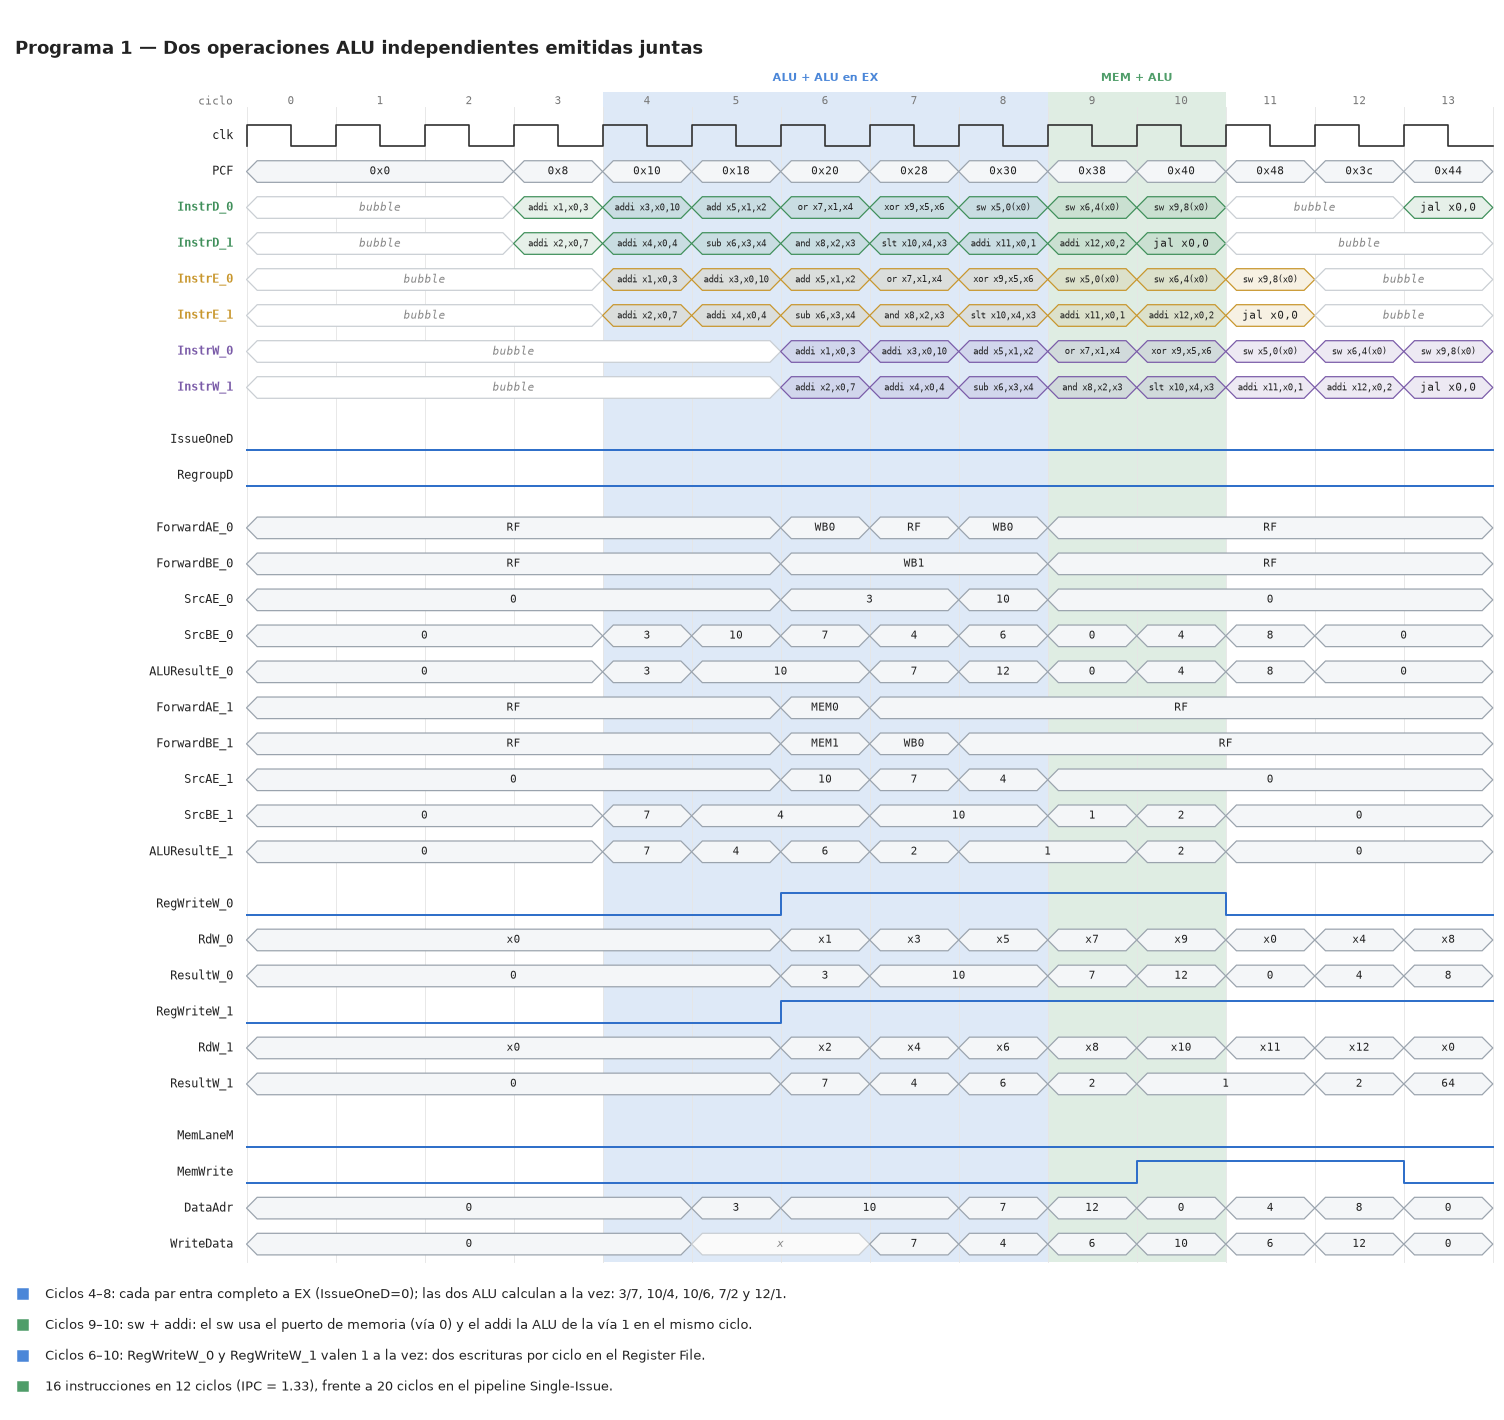
\includegraphics[width=\textwidth]{waveform-alu-pair}
  \caption{Waveform del Programa 1.}
  \label{fig:wave1}
\end{figure}

\textbf{Análisis.} Ningún par tiene dependencias internas, así que \texttt{IssueOneD} vale 0 todo el programa y cada par pasa completo a EX. Desde el ciclo 4 el PC avanza de 8 en 8 (\texttt{0x8}, \texttt{0x10}, \texttt{0x18}, ...). En los ciclos 4 a 8 las dos ALU trabajan a la vez: por ejemplo, en el ciclo 6 \texttt{add x5,x1,x2} calcula $3+7=10$ en la vía 0 y \texttt{sub x6,x3,x4} calcula $10-4=6$ en la vía 1. Aunque dentro de cada par no hay dependencias, sí las hay entre pares consecutivos, y se resuelven con forwarding desde ambas vías: en ese mismo ciclo \texttt{add x5} toma x1 de WB0 y x2 de WB1, y \texttt{sub x6} toma x3 de MEM0 y x4 de MEM1.

En los ciclos 9 y 10 se emiten pares \texttt{sw} + \texttt{addi}: el \texttt{sw} usa el puerto de memoria y el \texttt{addi} la ALU de la otra vía. Las escrituras en memoria (ciclos 10 a 12) son \texttt{MEM[0]}$=10$, \texttt{MEM[4]}$=6$ y \texttt{MEM[8]}$=12$, las esperadas. En WB, \texttt{RegWriteW\_0} y \texttt{RegWriteW\_1} se activan juntos desde el ciclo 6 y se escriben dos registros por ciclo (x1/x2, x3/x4, x5/x6, ...). El programa termina en 12 ciclos con 16 instrucciones (IPC $=1.33$); el pipeline necesita 20.

% ---------- PROGRAMA 2 ----------
\subsection{Programa 2: RAW dentro del par y forwarding entre vías}

\lstinputlisting[style=programa, caption={Programa 2 (\texttt{dualissue/raw\_forward.mem}).}]{../../tb/programs/dualissue/raw_forward.mem}

\begin{figure}[!htbp]
  \centering
  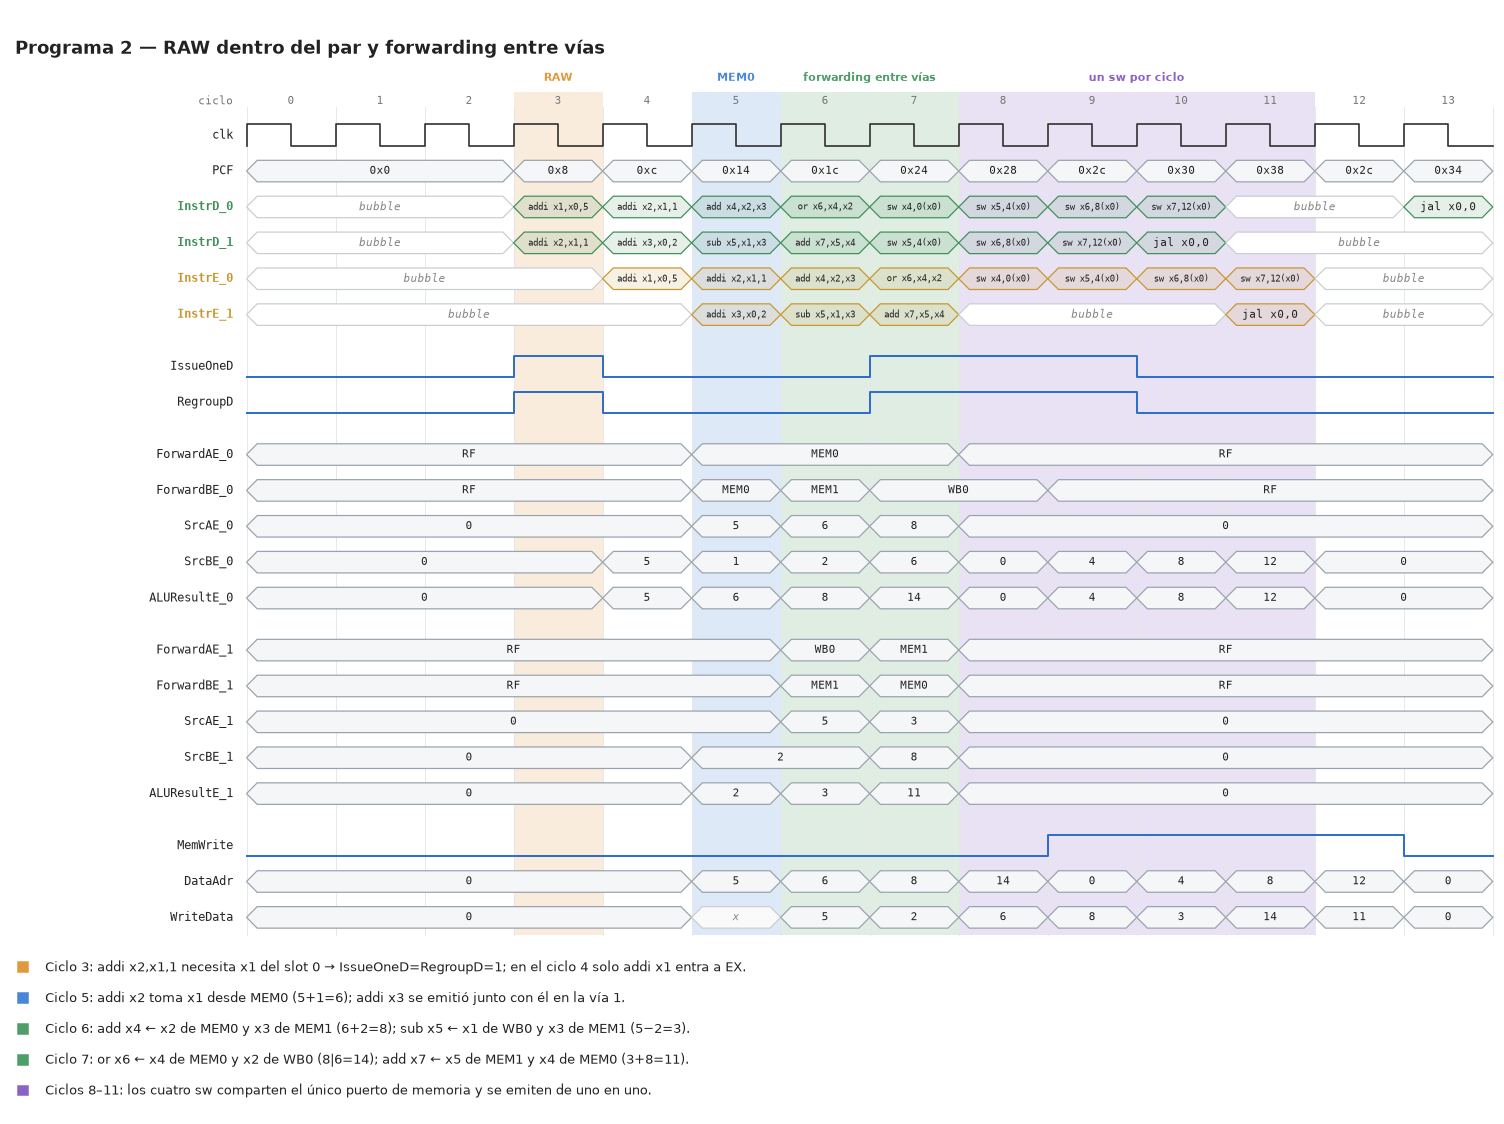
\includegraphics[width=\textwidth]{waveform-raw-forward}
  \caption{Waveform del Programa 2.}
  \label{fig:wave2}
\end{figure}

\textbf{Análisis.} En el ciclo 3 el par es (\texttt{addi x1,x0,5} | \texttt{addi x2,x1,1}). El slot 1 necesita x1, que el slot 0 recién calculará en EX, así que la Issue Unit activa \texttt{IssueOneD} y \texttt{RegroupD}. En el ciclo 4 solo \texttt{addi x1} entra a EX (\texttt{InstrE\_1} es burbuja) y en Decode se forma el par (\texttt{addi x2} | \texttt{addi x3}). En el ciclo 5 \texttt{addi x2} toma x1 desde MEM0 y calcula $5+1=6$.

En los ciclos 6 y 7 se ve el forwarding cruzado entre vías. En el ciclo 6, \texttt{add x4,x2,x3} (vía 0) toma x2 de MEM0 y x3 de MEM1, que fue producido por la otra vía, y da 8. \texttt{sub x5,x1,x3} (vía 1) toma x1 de WB0 y x3 de MEM1, y da 3. En el ciclo 7, \texttt{or x6,x4,x2} usa MEM0 y WB0 ($8 \lor 6 = 14$), y \texttt{add x7,x5,x4} usa MEM1 para x5 y MEM0 para x4 ($3+8=11$). Las cuatro combinaciones entre vías y etapas aparecen en el programa.

Al final hay cuatro \texttt{sw} seguidos. Como hay un solo puerto de memoria, \texttt{IssueOneD} vale 1 en los ciclos 7 a 9 y cada \texttt{sw} entra solo a EX. Las escrituras de los ciclos 9 a 12 son \texttt{MEM[0]}$=8$, \texttt{MEM[4]}$=3$, \texttt{MEM[8]}$=14$ y \texttt{MEM[12]}$=11$.

% ---------- PROGRAMA 3 ----------
\subsection{Programa 3: load-use y conflictos del puerto de memoria}

\lstinputlisting[style=programa, caption={Programa 3 (\texttt{dualissue/memory.mem}).}]{../../tb/programs/dualissue/memory.mem}

\begin{figure}[!htbp]
  \centering
  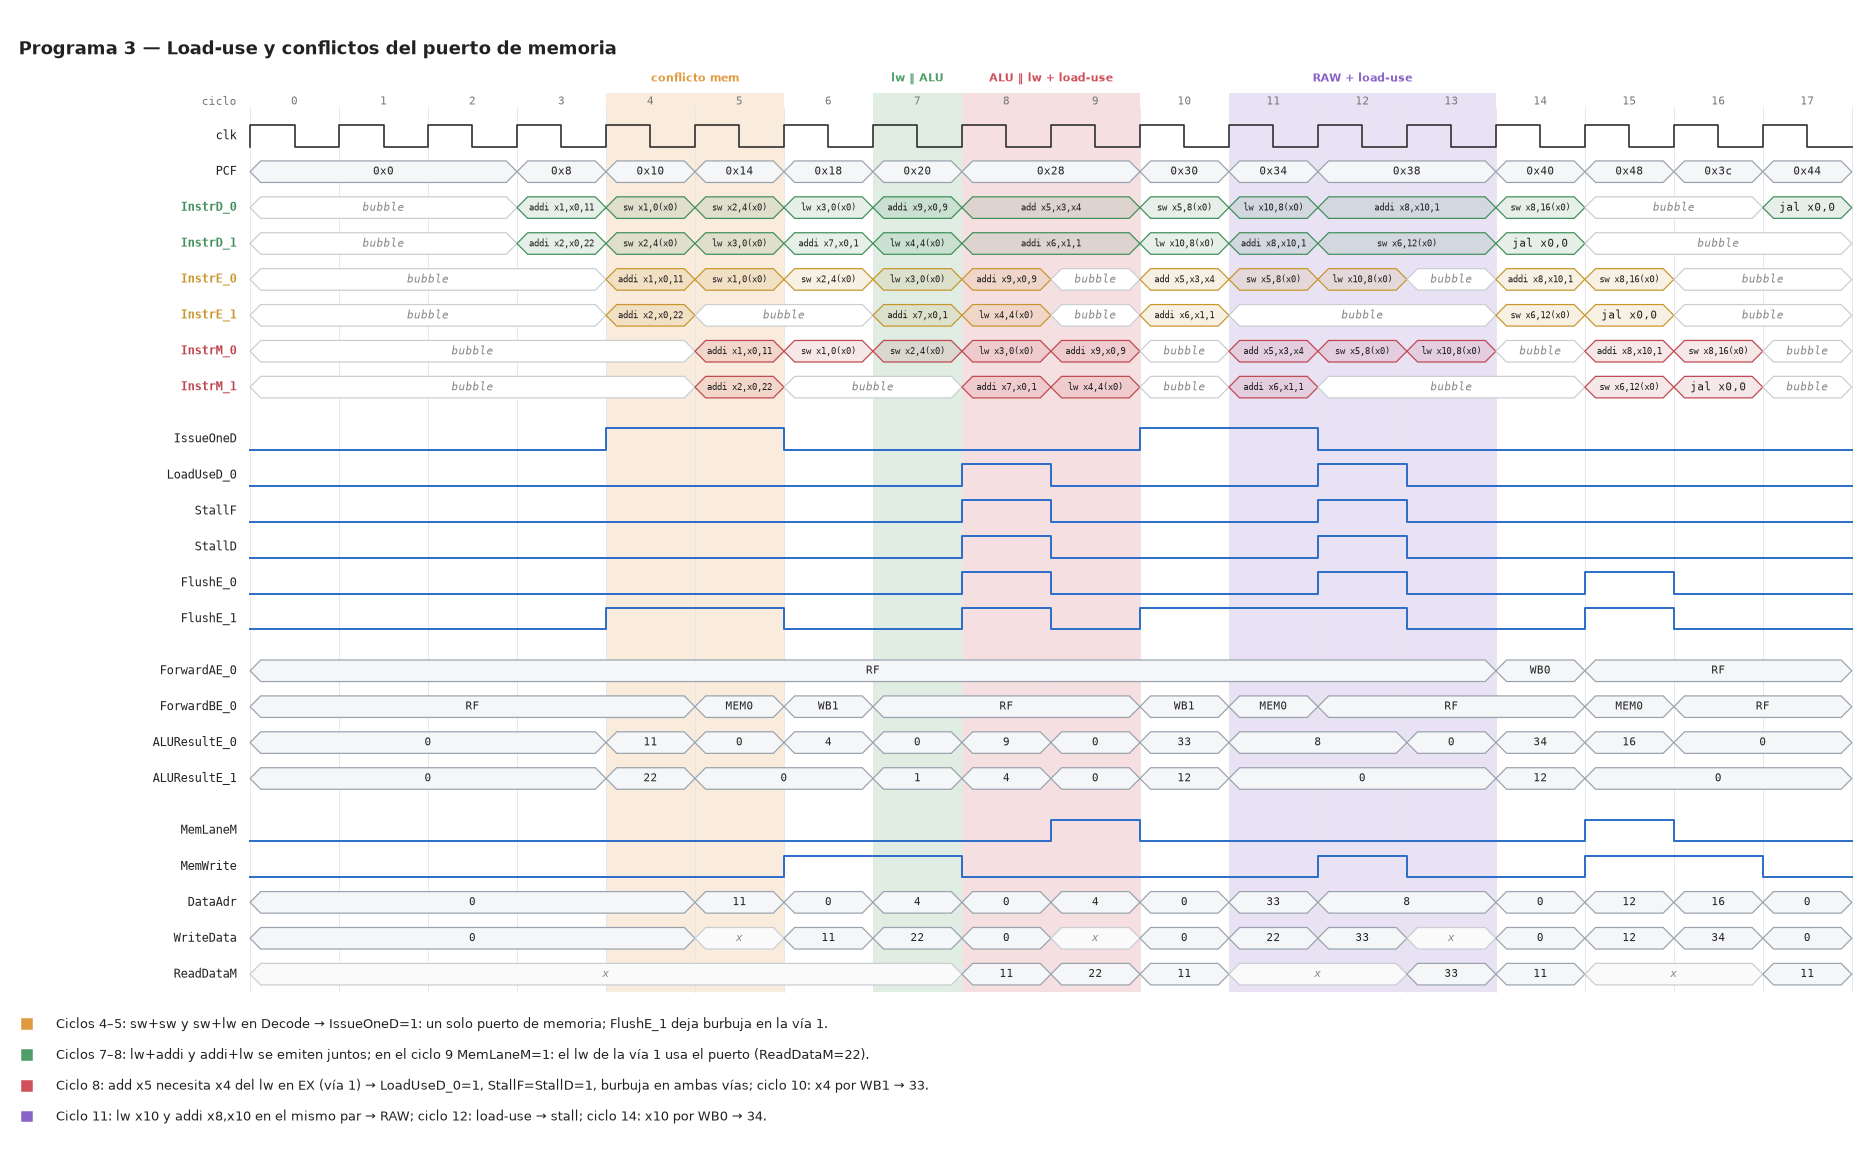
\includegraphics[width=\textwidth]{waveform-memory}
  \caption{Waveform del Programa 3.}
  \label{fig:wave3}
\end{figure}

\textbf{Análisis.} En los ciclos 4 y 5 Decode tiene los pares (\texttt{sw} | \texttt{sw}) y (\texttt{sw} | \texttt{lw}). Ambas instrucciones necesitan el puerto de memoria, por lo que \texttt{IssueOneD}$=1$ y se emiten en ciclos distintos (\texttt{FlushE\_1} deja la vía 1 vacía). En cambio, en el ciclo 7 entran juntos \texttt{lw x3} (vía 0) y \texttt{addi x7} (vía 1), y en el ciclo 8 \texttt{addi x9} (vía 0) y \texttt{lw x4} (vía 1). En el ciclo 9 \texttt{MemLaneM}$=1$: el puerto se asigna a la vía 1, la dirección es 4 y \texttt{ReadDataM}$=22$. Esto muestra que el orden ALU/memoria dentro del par no importa.

En el ciclo 8 \texttt{add x5,x3,x4} está en el slot 0 y necesita x4, que carga el \texttt{lw} de la vía 1 en EX. \texttt{LoadUseD\_0} se activa, \texttt{StallF} y \texttt{StallD} congelan el PC (\texttt{0x28}) y el par, y \texttt{FlushE\_0}/\texttt{FlushE\_1} ponen burbujas en ambas vías (ciclo 9). En el ciclo 10 el \texttt{lw x4} ya está en WB de la vía 1, y \texttt{add x5} toma x4 por WB1 ($11+22=33$).

El último caso combina las dos situaciones. En el ciclo 11 el par (\texttt{lw x10} | \texttt{addi x8,x10,1}) tiene RAW, así que solo se emite el \texttt{lw}. En el ciclo 12 \texttt{addi x8} ya es el slot 0 y el \texttt{lw} está en EX, lo que produce un stall. En el ciclo 14 \texttt{addi x8} toma x10 de WB0 y calcula 34. El programa tiene 2 stalls, igual que el pipeline. Las escrituras son \texttt{MEM[0]}$=11$, \texttt{MEM[4]}$=22$, \texttt{MEM[8]}$=33$, \texttt{MEM[12]}$=12$ (\texttt{sw} en la vía 1, ciclo 15) y \texttt{MEM[16]}$=34$.

% ---------- PROGRAMA 4 ----------
\subsection{Programa 4: branches en ambas posiciones y flushing}

\lstinputlisting[style=programa, caption={Programa 4 (\texttt{dualissue/branch.mem}).}]{../../tb/programs/dualissue/branch.mem}

\begin{landscape}
\begin{figure}[p]
  \centering
  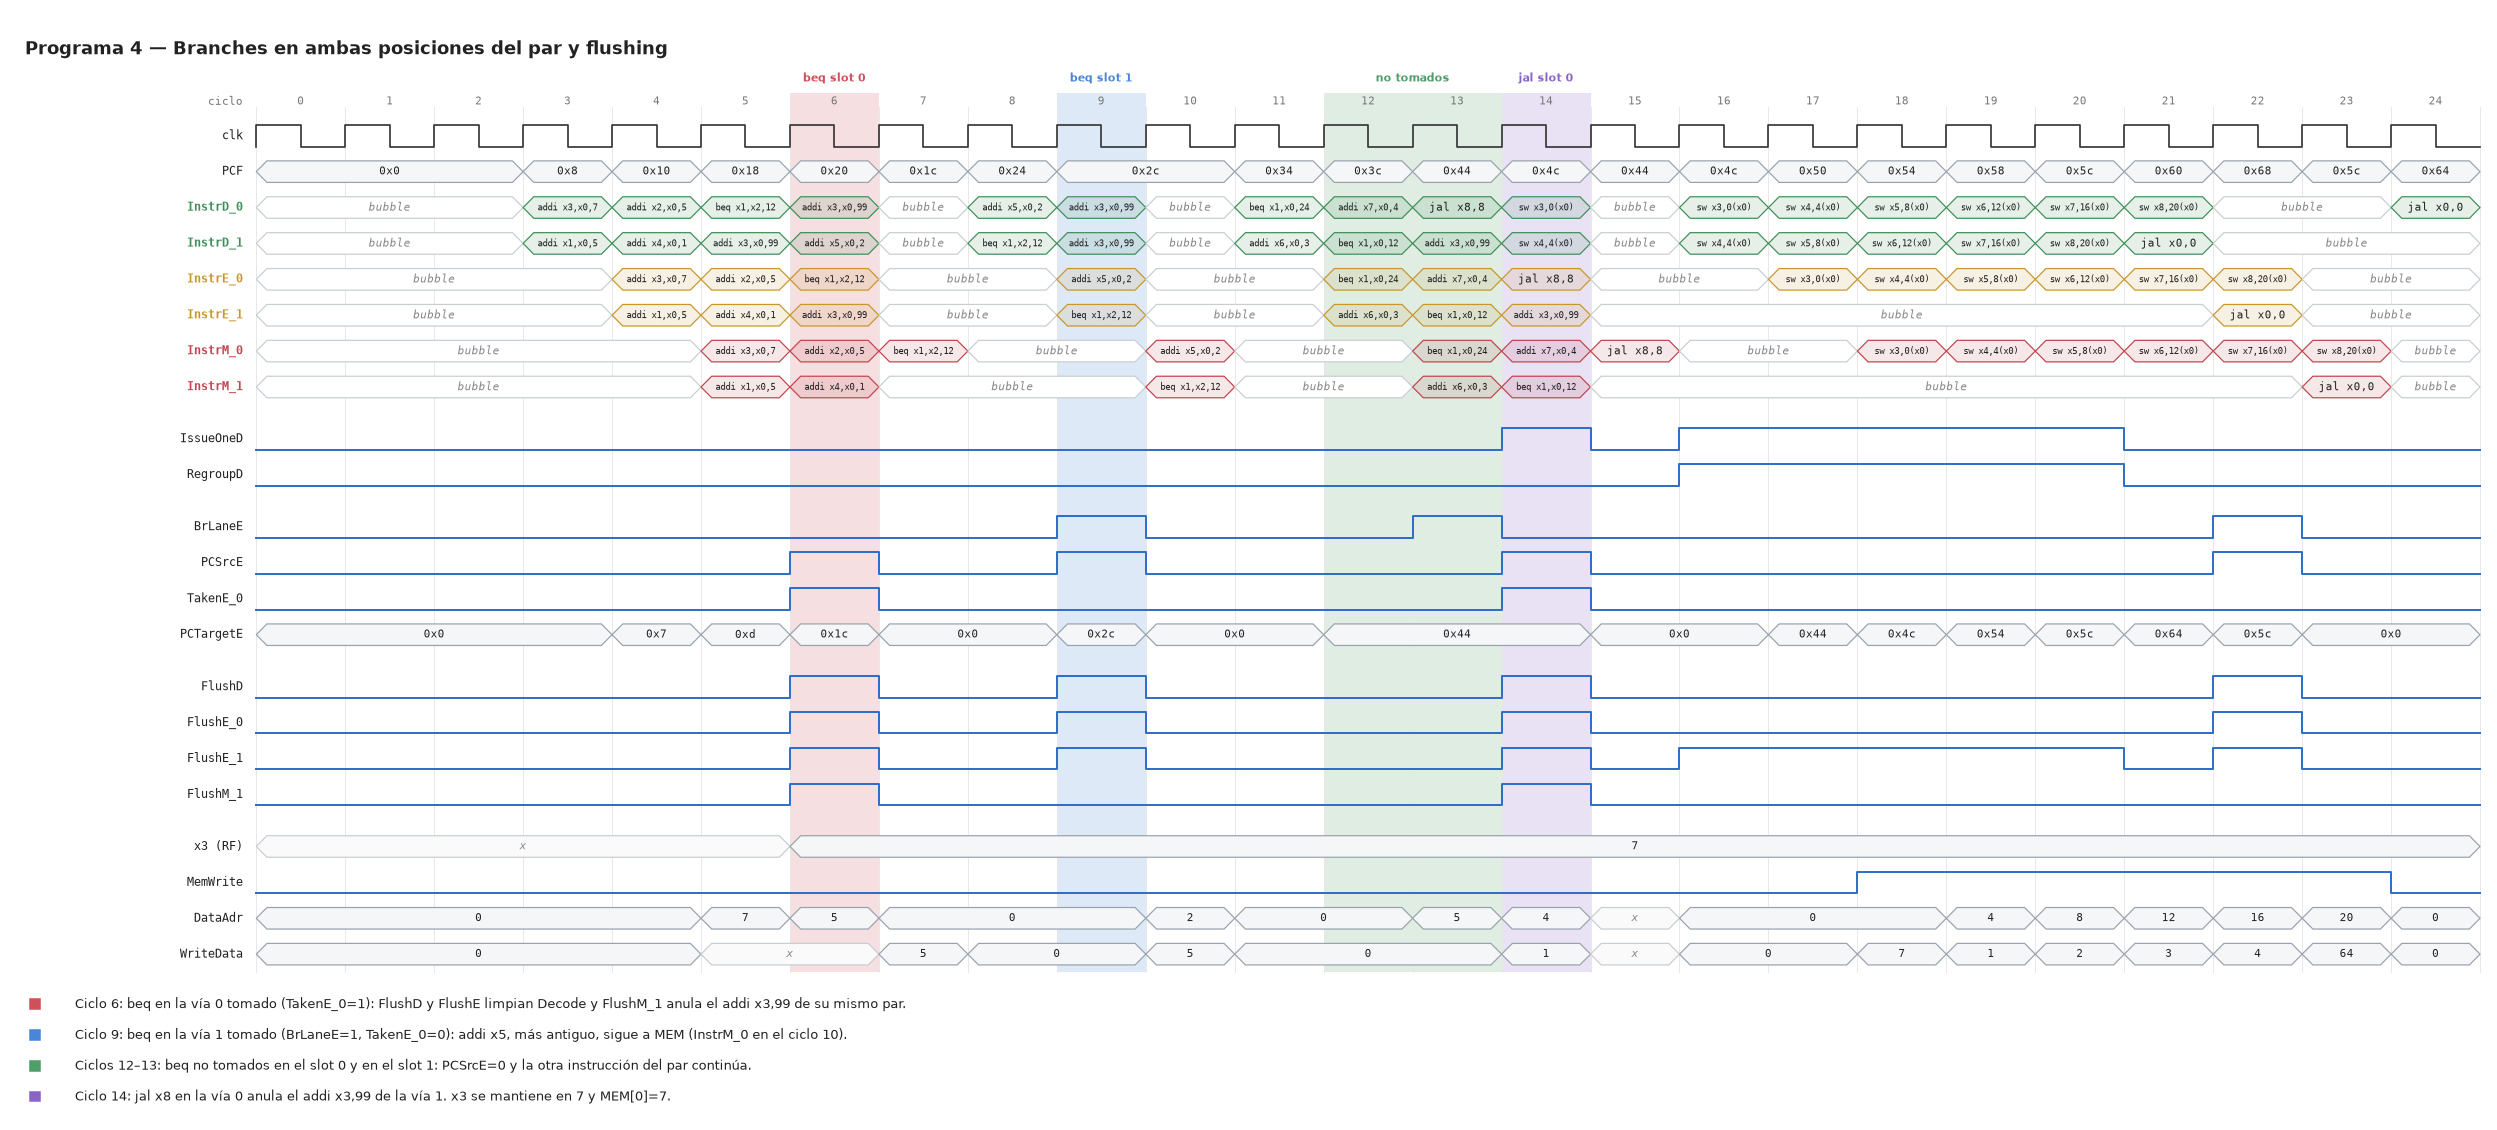
\includegraphics[width=\linewidth,height=0.82\textheight,keepaspectratio]{waveform-branch}
  \caption{Waveform del Programa 4.}
  \label{fig:wave4}
\end{figure}
\end{landscape}

\textbf{Análisis.} Las instrucciones del camino incorrecto escriben 99 en x3, así que si alguna llegara a WB, x3 dejaría de valer 7. La fila \texttt{x3 (RF)} se mantiene en 7 todo el programa.

\textit{Branch en el slot 0, tomado (ciclo 6).} \texttt{beq x1,x2,12} está en la vía 0 de EX junto con \texttt{addi x3,x0,99} en la vía 1. Se activan \texttt{PCSrcE} y \texttt{TakenE\_0}, y el PC salta a \texttt{0x1c}. \texttt{FlushD} y \texttt{FlushE} descartan las instrucciones de Decode, y \texttt{FlushM\_1} anula el \texttt{addi} del mismo par: en el ciclo 7 \texttt{InstrM\_1} es burbuja.

\textit{Branch en el slot 1, tomado (ciclo 9).} El par es (\texttt{addi x5,x0,2} | \texttt{beq x1,x2,12}). Ahora \texttt{BrLaneE}$=1$ y \texttt{TakenE\_0}$=0$, así que \texttt{FlushM\_1} no se activa y \texttt{addi x5}, que es más antigua, continúa a MEM (ciclo 10). Solo se descartan las instrucciones más jóvenes, que están en Decode. El PC salta a \texttt{0x2c}.

\textit{Branches no tomados (ciclos 12 y 13).} \texttt{beq x1,x0} no se cumple (x1$=5$). En el ciclo 12 está en el slot 0 y en el 13 en el slot 1 (\texttt{BrLaneE}$=1$). En ambos casos \texttt{PCSrcE}$=0$, la otra instrucción del par (\texttt{addi x6}, \texttt{addi x7}) se ejecuta normalmente y el PC sigue avanzando de 8 en 8.

\textit{jal en el slot 0 (ciclo 14).} \texttt{jal x8,8} es un salto incondicional en la vía 0: anula el \texttt{addi x3,99} de su par (\texttt{FlushM\_1}) y guarda la dirección de retorno $x8=64$. Al final se escriben \texttt{MEM[0]}$=7$, \texttt{[4]}$=1$, \texttt{[8]}$=2$, \texttt{[12]}$=3$, \texttt{[16]}$=4$ y \texttt{[20]}$=64$, todos correctos.

% ---------- PROGRAMA 5 ----------
\subsection{Programa 5: dos escrituras en el Register File}

\lstinputlisting[style=programa, caption={Programa 5 (\texttt{dualissue/two\_writes.mem}).}]{../../tb/programs/dualissue/two_writes.mem}

\begin{figure}[!htbp]
  \centering
  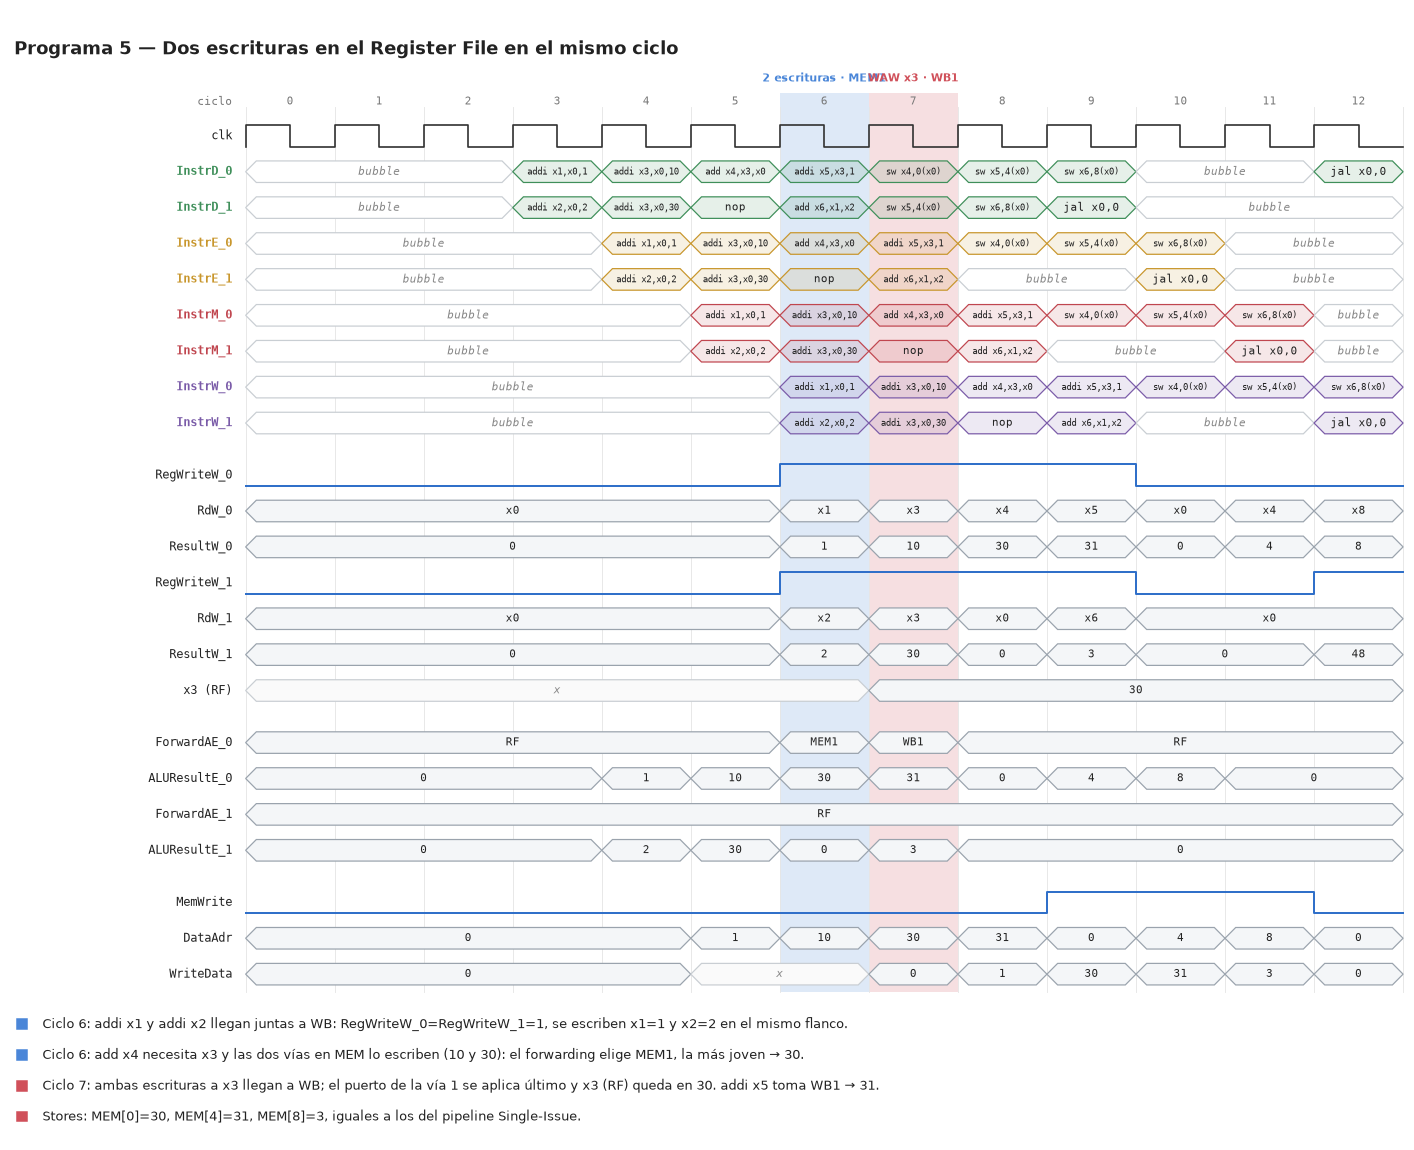
\includegraphics[width=\textwidth]{waveform-two-writes}
  \caption{Waveform del Programa 5.}
  \label{fig:wave5}
\end{figure}

\textbf{Análisis.} En el ciclo 6 los dos \texttt{addi} del primer par llegan juntos a WB: \texttt{RegWriteW\_0}$=$\texttt{RegWriteW\_1}$=1$, con x1$=1$ por el puerto de la vía 0 y x2$=2$ por el de la vía 1, en el mismo flanco de bajada.

El segundo par escribe el mismo registro (\texttt{addi x3,x0,10} | \texttt{addi x3,x0,30}). Como no hay RAW, se emite junto, y el valor correcto es el de la instrucción más joven, 30. Esto se cumple en tres lugares:
\begin{itemize}
    \item \textbf{Forwarding desde MEM (ciclo 6):} \texttt{add x4,x3,x0} encuentra x3 en MEM0 y MEM1 a la vez; la prioridad elige MEM1 y \texttt{ALUResultE\_0}$=30$.
    \item \textbf{Escritura (ciclo 7):} ambos puertos escriben x3 (\texttt{ResultW\_0}$=10$, \texttt{ResultW\_1}$=30$); el de la vía 1 se aplica último y \texttt{x3 (RF)} queda en 30.
    \item \textbf{Forwarding desde WB (ciclo 7):} \texttt{addi x5,x3,1} encuentra x3 en WB0 y WB1; elige WB1 y calcula 31.
\end{itemize}
Las escrituras en memoria son \texttt{MEM[0]}$=30$, \texttt{MEM[4]}$=31$ y \texttt{MEM[8]}$=3$.

% ---------- PROGRAMA 6 ----------
\subsection{Programa 6: reagrupamiento y orden del programa}

\lstinputlisting[style=programa, caption={Programa 6 (\texttt{dualissue/regroup.mem}).}]{../../tb/programs/dualissue/regroup.mem}

\begin{figure}[!htbp]
  \centering
  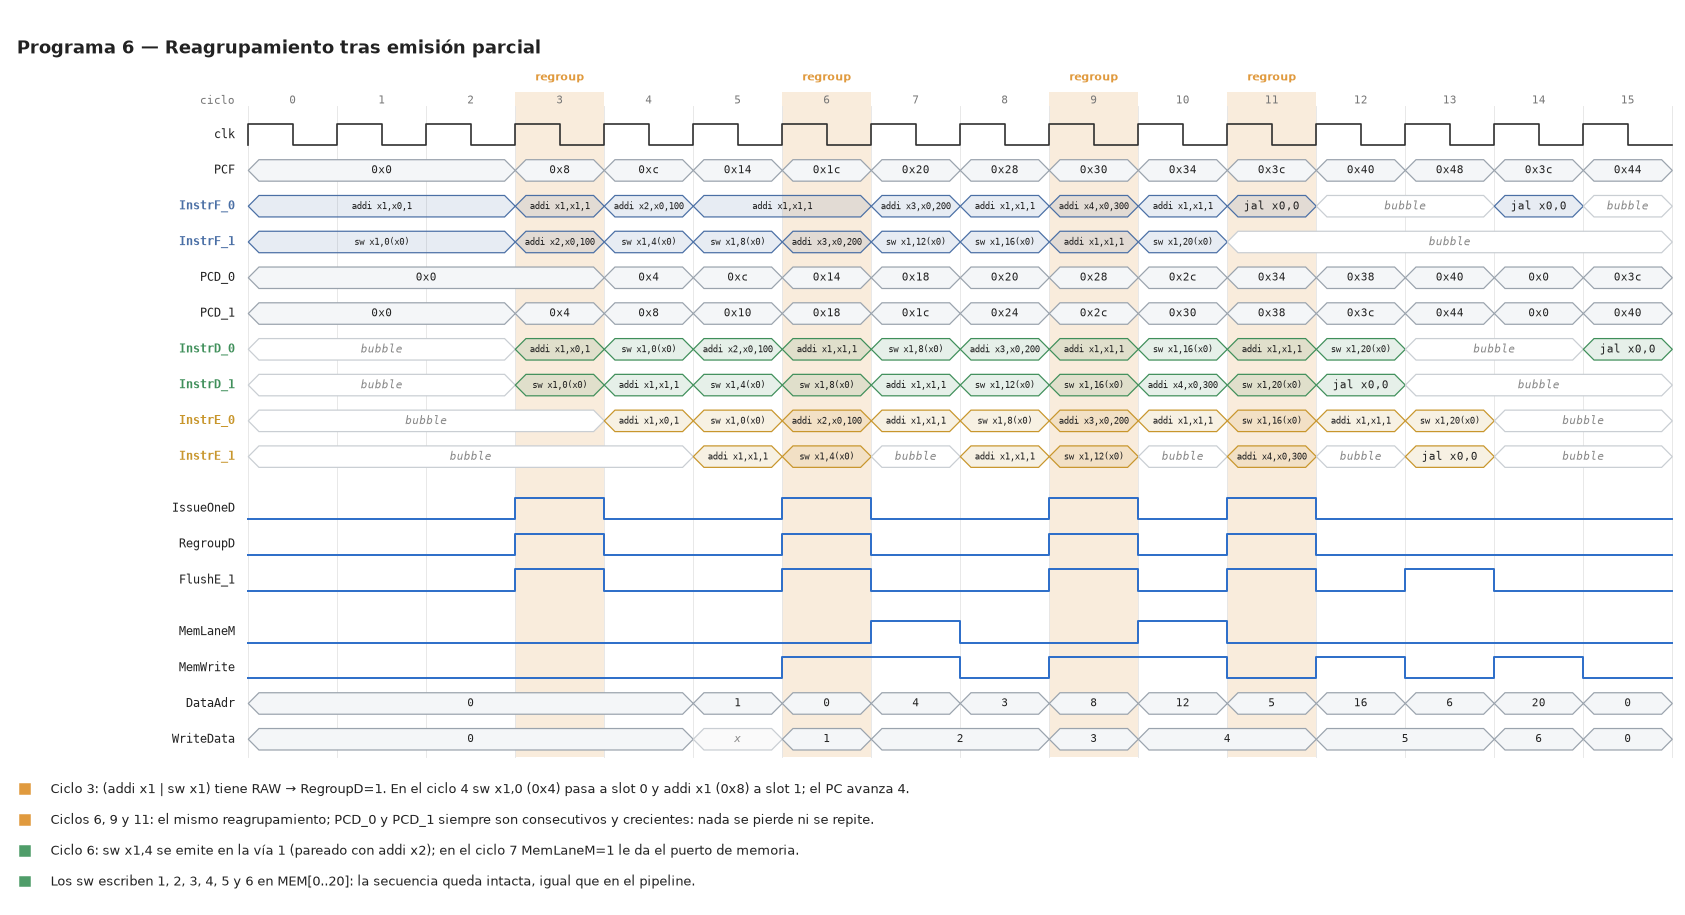
\includegraphics[width=\textwidth]{waveform-regroup}
  \caption{Waveform del Programa 6.}
  \label{fig:wave6}
\end{figure}

\textbf{Análisis.} El programa alterna una cadena de incrementos dependientes de x1 con instrucciones independientes, de modo que muchos pares no pueden emitirse completos. En el ciclo 3 el par es (\texttt{addi x1,x0,1} @\texttt{0x0} | \texttt{sw x1,0(x0)} @\texttt{0x4}) y tiene RAW. \texttt{RegroupD}$=1$, el PC avanza solo 4 (\texttt{0x8}$\to$\texttt{0xc}) y en el ciclo 4 el nuevo par es (\texttt{sw x1,0} @\texttt{0x4} | \texttt{addi x1,x1,1} @\texttt{0x8}): la instrucción que esperaba pasó al slot 0 y la primera que se buscó (\texttt{InstrF\_0} del ciclo 3) pasó al slot 1. Ese par se emite completo en el ciclo 5.

El reagrupamiento se repite en los ciclos 6, 9 y 11. En todo momento \texttt{PCD\_1}$=$\texttt{PCD\_0}$+4$ y los valores de \texttt{PCD\_0} solo crecen (\texttt{0x0}, \texttt{0x4}, \texttt{0xc}, \texttt{0x14}, \texttt{0x18}, ...), sin saltos ni repeticiones, lo que confirma que no se pierden ni se duplican instrucciones. También se observa un \texttt{sw} en el slot 1: en el ciclo 6 \texttt{sw x1,4(x0)} entra a EX por la vía 1, toma x1 de MEM1 y en el ciclo 7 usa el puerto de memoria (\texttt{MemLaneM}$=1$).

Cada \texttt{sw} guarda el valor actual de x1, así que una instrucción perdida o repetida cambiaría la secuencia guardada. \texttt{WriteData} toma los valores 1, 2, 3, 4, 5 y 6, en ese orden y en las direcciones 0 a 20.

% ---------- PROGRAMA 7 ----------
\subsection{Programa 7: conflicto en la Branch Unit y jal en el slot 1}

Este programa completa los casos de control: dos saltos en el mismo par, un \texttt{jal} tomado en el slot 1 y un \texttt{beq} que depende de la otra instrucción de su par.

\lstinputlisting[style=programa, caption={Programa 7 (\texttt{dualissue/branch\_conflict.mem}).}]{../../tb/programs/dualissue/branch_conflict.mem}

\begin{landscape}
\begin{figure}[p]
  \centering
  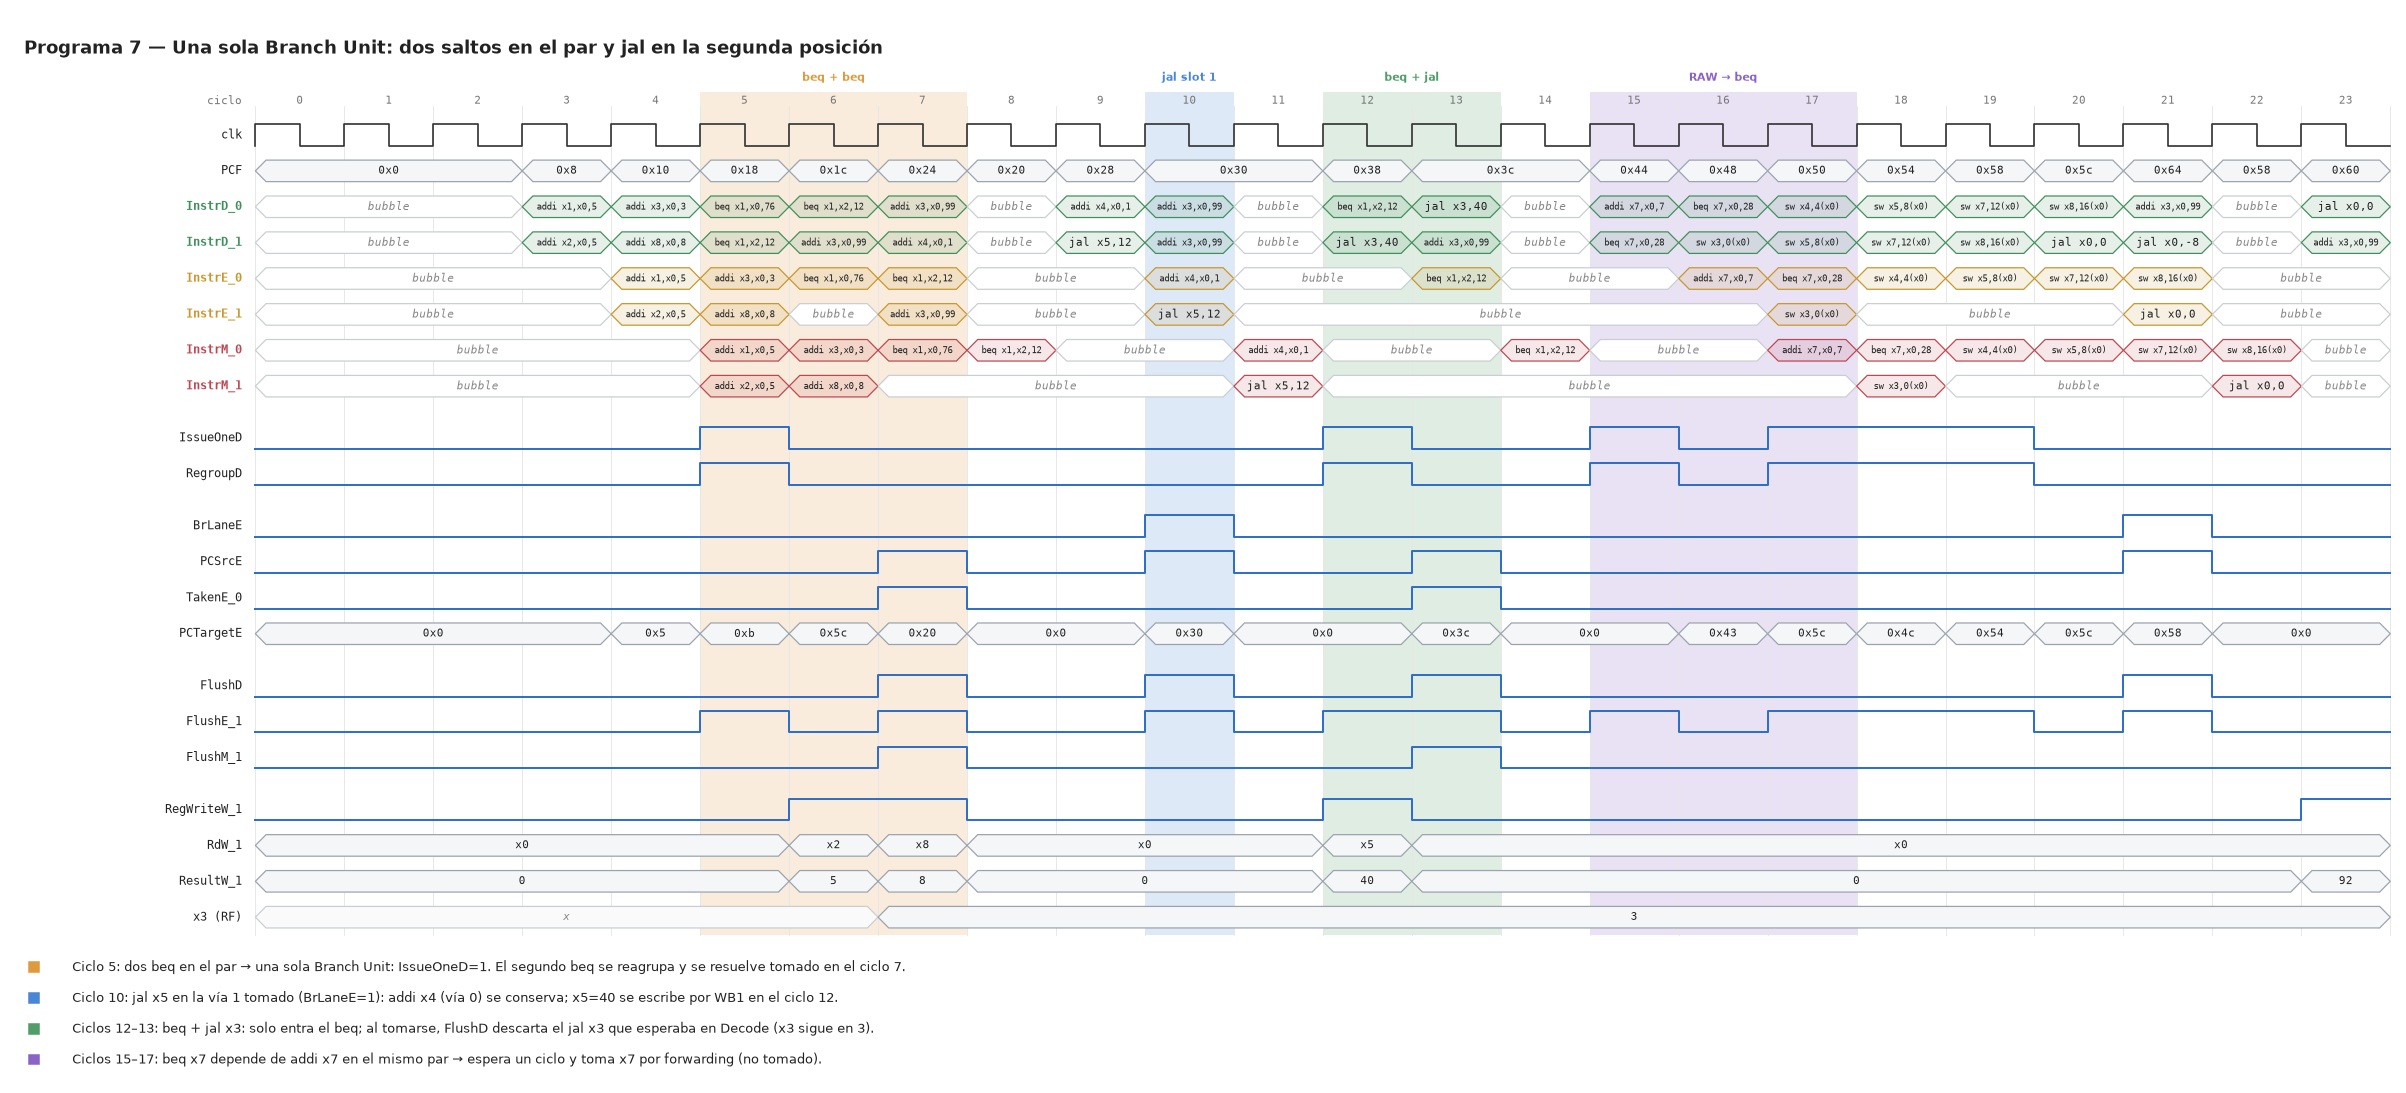
\includegraphics[width=\linewidth,height=0.82\textheight,keepaspectratio]{waveform-branch-conflict}
  \caption{Waveform del Programa 7.}
  \label{fig:wave7}
\end{figure}
\end{landscape}

\textbf{Análisis.} En el ciclo 5 el par es (\texttt{beq x1,x0} | \texttt{beq x1,x2}). Como hay una sola Branch Unit, \texttt{IssueOneD}$=1$ y solo pasa el primero (no tomado, ciclo 6). El segundo se reagrupa como slot 0, entra a EX en el ciclo 7 y se toma: el PC va a \texttt{0x20}, se limpia Decode y \texttt{FlushM\_1} anula el \texttt{addi x3,99} que lo acompañaba en la vía 1.

En el ciclo 10 el par en EX es (\texttt{addi x4} | \texttt{jal x5,12}). El salto está en la vía 1 (\texttt{BrLaneE}$=1$, \texttt{TakenE\_0}$=0$), así que \texttt{addi x4} se conserva y llega a MEM en el ciclo 11. El \texttt{jal} escribe su dirección de retorno por la vía 1: \texttt{RdW\_1}$=$x5, \texttt{ResultW\_1}$=40$ en el ciclo 12.

En el ciclo 12 el par (\texttt{beq x1,x2} | \texttt{jal x3,40}) vuelve a tener dos saltos y solo entra el \texttt{beq}. En el ciclo 13 el \texttt{beq} se toma y \texttt{FlushD} descarta el \texttt{jal x3} que esperaba en Decode. Ese \texttt{jal} habría escrito x3, pero x3 se mantiene en 3. Por último, en el ciclo 15 \texttt{beq x7,x0} depende de \texttt{addi x7} en el mismo par: espera un ciclo, entra a EX en el ciclo 17 con x7 adelantado desde MEM0 y no se toma. Las escrituras son \texttt{MEM[0]}$=3$, \texttt{[4]}$=1$, \texttt{[8]}$=40$, \texttt{[12]}$=7$ y \texttt{[16]}$=8$.

\subsection{Resumen de señales}

\begin{table}[H]
\centering
\small
\begin{tabularx}{\linewidth}{lX}
\toprule
\textbf{Señal} & \textbf{Qué indica} \\
\midrule
\texttt{InstrF/D/E/M/W\_0/1} & Instrucción en cada etapa y vía (solo para depurar). \\
\texttt{PCD\_0}, \texttt{PCD\_1} & Dirección de cada slot del par en Decode. \\
\texttt{IssueOneD} & La Issue Unit solo deja pasar el slot 0. \\
\texttt{LoadUseD\_0} & El slot 0 depende de un \texttt{lw} en EX (stall). \\
\texttt{RegroupD} & El slot 1 pasa a slot 0; el PC avanza 4. \\
\texttt{StallF}, \texttt{StallD} & Congelan el PC y el IF/ID. \\
\texttt{FlushD}, \texttt{FlushE\_0/1}, \texttt{FlushM\_1} & Anulan Decode, EX de cada vía y MEM de la vía 1. \\
\texttt{ForwardAE/BE\_0/1} & Fuente de cada operando: RF, WB0, WB1, MEM0 o MEM1. \\
\texttt{SrcAE/SrcBE/ALUResultE\_0/1} & Operandos y resultado de cada ALU. \\
\texttt{BrLaneE}, \texttt{PCSrcE}, \texttt{TakenE\_0}, \texttt{PCTargetE} & Vía del salto en EX, si se toma, si está en la vía 0 y a dónde va. \\
\texttt{MemLaneM}, \texttt{MemWrite}, \texttt{DataAdr}, \texttt{WriteData}, \texttt{ReadDataM} & Vía dueña del puerto de memoria y el acceso. \\
\texttt{RegWriteW/RdW/ResultW\_0/1} & Las dos escrituras en el Register File. \\
\bottomrule
\end{tabularx}
\caption{Señales observadas en las waveforms.}
\label{tab:senales}
\end{table}

\FloatBarrier
% =====================================================================
\section{Comparación preliminar frente al Single-Issue}
\label{sec:comp}

\subsection{Metodología}

Ambos diseños se simulan con el mismo testbench (\texttt{tb/perf\_tb.v}; el Dual-Issue se compila con \texttt{-DDUAL}) y los mismos programas, sin modificarlos. El criterio de medición es el mismo en los dos: se cuenta desde el primer ciclo después del reset hasta el ciclo en que el \textit{halt} (\texttt{jal x0,0}) llega a WB. Las instrucciones retiradas son las que llegan a WB (sin contar burbujas), incluido el \textit{halt}. El script \texttt{tb/run\_all.sh} ejecuta todos los programas en las dos arquitecturas, compara el estado final (los 31 registros y la memoria de datos) y calcula las métricas:
\begin{equation*}
\text{IPC} = \frac{\text{instrucciones}}{\text{ciclos}}, \qquad
\text{CPI} = \frac{\text{ciclos}}{\text{instrucciones}}, \qquad
\text{Speedup}_{A\to B} = \frac{\text{ciclos}(A)}{\text{ciclos}(B)}
\end{equation*}

Además de los programas de esta entrega se incluyen los cuatro de E1 y un pequeño benchmark, \texttt{loop.mem}, que llena un arreglo de 8 palabras con un bucle y luego lo suma con otro (\texttt{lw}, \texttt{add}, \texttt{beq}, \texttt{jal}).

\subsection{Resultados}

\begin{table}[H]
\centering
\footnotesize
\setlength{\tabcolsep}{3.5pt}
\begin{tabular}{@{}lccccccccccc@{}}
\toprule
 & & \multicolumn{2}{c}{\textbf{A: Pipeline}} & \multicolumn{3}{c}{\textbf{B: Dual-Issue}} & \multicolumn{4}{c}{\textbf{Eventos en B (ciclos)}} & \\
\cmidrule(lr){3-4} \cmidrule(lr){5-7} \cmidrule(lr){8-11}
\textbf{Programa} & \textbf{Instr.} & \textbf{Ciclos} & \textbf{IPC} & \textbf{Ciclos} & \textbf{IPC} & \textbf{CPI} & \textbf{Dual} & \textbf{Regr.} & \textbf{Stall} & \textbf{Flush} & \textbf{Speedup} \\
\midrule
P1 \texttt{alu\_pair}        & 16 & 20 & 0.800 & 12 & 1.333 & 0.750 &  8 & 0 & 0 & 1 & 1.667 \\
P2 \texttt{raw\_forward}     & 12 & 16 & 0.750 & 12 & 1.000 & 1.000 &  4 & 4 & 0 & 1 & 1.333 \\
P3 \texttt{memory}           & 16 & 22 & 0.727 & 16 & 1.000 & 1.000 &  6 & 4 & 2 & 1 & 1.375 \\
P4 \texttt{branch}           & 19 & 29 & 0.655 & 23 & 0.826 & 1.211 &  8 & 5 & 0 & 4 & 1.261 \\
P5 \texttt{two\_writes}      & 12 & 16 & 0.750 & 11 & 1.091 & 0.917 &  5 & 2 & 0 & 1 & 1.455 \\
P6 \texttt{regroup}          & 16 & 20 & 0.800 & 14 & 1.143 & 0.875 &  6 & 4 & 0 & 1 & 1.429 \\
P7 \texttt{branch\_conflict} & 17 & 27 & 0.630 & 22 & 0.773 & 1.294 &  6 & 6 & 0 & 4 & 1.227 \\
\midrule
E1 \texttt{isa}              & 14 & 18 & 0.778 & 13 & 1.077 & 0.929 &  5 & 4 & 0 & 1 & 1.385 \\
E1 \texttt{forwarding}       &  8 & 12 & 0.667 & 11 & 0.727 & 1.375 &  1 & 6 & 0 & 1 & 1.091 \\
E1 \texttt{stall}            &  9 & 15 & 0.600 & 14 & 0.643 & 1.556 &  1 & 7 & 2 & 1 & 1.071 \\
E1 \texttt{flush}            &  8 & 16 & 0.500 & 14 & 0.571 & 1.750 &  4 & 2 & 0 & 3 & 1.143 \\
\midrule
\texttt{loop} (benchmark)    & 89 & 129 & 0.690 & 93 & 0.957 & 1.045 & 45 & 8 & 0 & 19 & 1.387 \\
\bottomrule
\end{tabular}
\caption{Ciclos, IPC y speedup del Dual-Issue (B) frente al pipeline Single-Issue (A). \textit{Dual}: ciclos con dos instrucciones en EX; \textit{Regr.}: ciclos con reagrupamiento; \textit{Flush}: ciclos con \texttt{FlushD} (incluye el \textit{halt}).}
\label{tab:comp}
\end{table}

En los 12 programas, \texttt{run\_all.sh} reporta \textbf{OK}: el pipeline y el Dual-Issue terminan con los mismos registros y la misma memoria de datos.

\subsection{Análisis}

El Dual-Issue es más rápido en todos los programas, con speedups entre 1.07 y 1.67. La mejora depende de cuánto paralelismo tenga cada programa:

\begin{itemize}
    \item \textbf{Instrucciones independientes.} En P1 casi todos los pares se emiten juntos (8 ciclos con dos instrucciones en EX) y se obtiene el mayor speedup, 1.67. Aun así, el IPC es 1.33 y no 2, porque los programas son cortos y los 4 ciclos de llenado del pipeline y el \textit{halt} pesan mucho: 16 instrucciones necesitan al menos $8 + 4 = 12$ ciclos.
    \item \textbf{Dependencias.} Los programas de E1 \texttt{forwarding} y \texttt{stall} son cadenas en las que cada instrucción depende de la anterior. Casi ningún par puede emitirse completo (6 y 7 reagrupamientos), así que el Dual-Issue se comporta como el pipeline (speedup de 1.09 y 1.07). El paralelismo disponible lo limita el programa, no el hardware.
    \item \textbf{Recursos compartidos.} Los \texttt{sw} consecutivos de P2, P3 y P4 se emiten de a uno por el único puerto de memoria. P7 pierde ciclos adicionales porque dos saltos no pueden ir en el mismo par.
    \item \textbf{Saltos.} Es la limitación más importante en código con bucles. En \texttt{loop} hay 19 saltos tomados (18 del bucle más el \textit{halt}), cada uno resuelto en EX con 2 ciclos perdidos: unos 38 de los 93 ciclos se pierden por flush. Por eso el IPC queda en 0.96 aunque en 45 ciclos se ejecutan dos instrucciones a la vez. En el pipeline un salto tomado desperdicia 2 instrucciones; en el Dual-Issue desperdicia hasta 4.
\end{itemize}

En resumen, el procesador aprovecha el paralelismo cuando el código lo permite. Lo que impide acercarse al IPC ideal de 2 son, en este orden, los saltos tomados, las dependencias RAW entre instrucciones vecinas y los conflictos en los recursos compartidos. Estas mediciones servirán como referencia (arquitectura B) para evaluar la optimización de la entrega final.

\section{Conclusiones}

\begin{itemize}
    \item Se completó el procesador Dual-Issue In-Order: dos vías con ALU propia hasta WB, Register File de 4 lecturas y 2 escrituras, un único puerto de memoria y una única Branch Unit, ambos asignados dinámicamente a la vía que los necesita.
    \item La Issue Unit emite dos instrucciones, una o ninguna según RAW dentro del par, conflictos de memoria o de saltos y load-use. Cuando emite solo una, el reagrupamiento combina la instrucción pendiente con la siguiente sin perder ni repetir instrucciones.
    \item La Hazard Unit adelanta datos desde las dos vías en MEM y WB, con prioridad para el productor más joven, y anula únicamente las instrucciones más jóvenes que un salto tomado, conservando la instrucción más antigua cuando el salto está en el slot 1.
    \item Los siete programas de prueba y los cuatro de E1 producen el mismo estado final en el pipeline y en el Dual-Issue. El speedup va de 1.07 a 1.67, y los saltos tomados son la principal causa de pérdida de rendimiento.
\end{itemize}

\end{document}
